\chapter{Практическая часть}

В листинге 3.1 представлена реализация информационного центра на
языке имитационного моделирования GPSS.

\begin{lstlisting}[caption=Реализация системы массового обслуживания]
			GENERATE 		10 ,2 ,0 ,300
operator_1  GATE NU 		oper_1 , operator_2
			SEIZE 			oper_1
			ADVANCE 		20 ,5
			RELEASE 		oper_1
			TRANSFER 		,computer_1
operator_2  GATE NU 		oper_2 , operator_3
			SEIZE 			oper_2
			ADVANCE 		40 ,10
			RELEASE 		oper_2
			TRANSFER 		,computer_1
operator_3  GATE NU 		oper_3 , fail
			SEIZE			oper_3
			ADVANCE 		40 ,20
			RELEASE 		oper_3
		    TRANSFER 		,computer_2
computer_1  QUEUE 			queue_1
			SEIZE 			comp_1
			DEPART 			queue_1
			ADVANCE 		15
			RELEASE 		comp_1
			TRANSFER 		,success
computer_2  QUEUE		 	queue_2
			SEIZE 			comp_2
			DEPART 			queue_2
			ADVANCE 		30
			RELEASE 		comp_2
			TRANSFER 		,success
success 	TRANSFER 		,ending
fail 		TRANSFER 		,ending
ending 		SAVEVALUE nfail , n$fail
			SAVEVALUE prob ,(( n$fail ) /( n$success + n$fail ))
			TERMINATE 1
			START 300
\end{lstlisting}

На рисунке 3.1 демонстрируется работа программы. Вероятность отказа равна 47\%.

\begin{figure}[h]
	\centering
	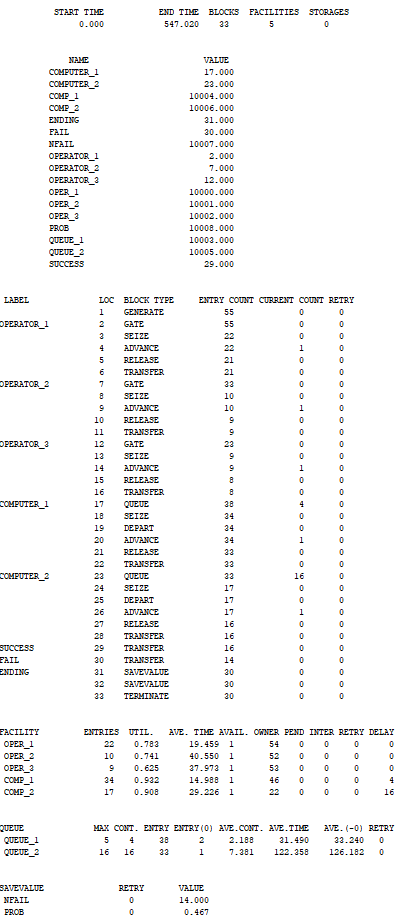
\includegraphics[height=0.96\textheight]{img/res.png}
	\caption{Отчёт информационного центра}
	\label{plt:even_comp_alg}
\end{figure}
